% ========================
% = Rapport de projet HA =
% ========================
% Joris Berthelot <joris.berthelot@gmail.com>
% Laurent Le Moine <laurent.le.moine17@gmail.com>
% 


\documentclass[11pt,a4paper]{report}
\usepackage{
    content/fullpage, % Enclosed as .sty file
    hyperref,
    listings,
    lmodern,
    soul,
    fancyhdr,
    algorithmic,
    minted % How to install: http://blog.eexit.net/2011/02/latex-colorez-efficacement-votre-code-source-avec-minted.html
}
%\usepackage[utf8]{inputenc}
\usepackage[T1]{fontenc}
\usepackage[french]{babel}
\usepackage[pdftex]{graphicx}
\pagestyle{fancyplain}
\fancyhf{}
\lhead{\fancyplain{}{Dossier d'Architecture Technique}}
\rhead{\fancyplain{}{Universit\'e de La Rochelle}}
\lfoot{\fancyplain{}{Joris \textsc{BERTHELOT} - Laurent \textsc{LE MOINE}}}
\rfoot{\fancyplain{}{\thepage}}
\definecolor{lightgray}{gray}{.95}
\usemintedstyle{manni}
\newminted{bash}{
    linenos=false,
    bgcolor=lightgray,
    tabsize=4,
    gobble=20,
    fontfamily=courier,
    fontsize=\small,
    xleftmargin=5pt,
    xrightmargin=5pt
}
\hypersetup{
    bookmarks=true,
    unicode=true,
    pdfstartview={FitW}
    pdftitle={Dossier d'Architecture Technique},
    pdfauthor={Joris Berthelot, Laurent Le Moine},
    pdfnewwindow=true,
    colorlinks=true,
    citecolor=black,
    filecolor=black,
    linkcolor=black,
    urlcolor=black
}
\begin{document}
    \newcommand{\HRule}{\rule{\linewidth}{0.5mm}}

\begin{titlepage}

\begin{center}


% Upper part of the page

\includegraphics[width=0.15\textwidth]{content/logo.png}\\[1cm]

\textsc{\LARGE Universit\'e de La Rochelle}\\[1.5cm]

\textsc{\Large Rapport de projet}\\[0.5cm]


% Title
\HRule \\[0.4cm]
{ \huge \bfseries Dossier d'Architecture Technique}\\[0.4cm]

\HRule \\[1.5cm]

% Author and supervisor
\begin{minipage}{0.4\textwidth}
    \begin{flushleft} \large
        \emph{Auteurs:}\\
        Joris \textsc{BERTHELOT}\\
        Laurent \textsc{LE MOINE}
    \end{flushleft}
\end{minipage}
\begin{minipage}{0.4\textwidth}
    \begin{flushright} \large
        \emph{Superviseurs:} \\
        Philippe \textsc{HARRAND}\\
        Bertrand \textsc{VACHON}
    \end{flushright}
\end{minipage}

\vfill

% Bottom of the page
{Master ICONE 2011-2012}

\end{center}

\end{titlepage}
    \newpage
    \setcounter{secnumdepth}{3}
    \setcounter{tocdepth}{4}
    \tableofcontents
    \newpage
    
        \section*{Introduction}
        
        \addcontentsline{toc}{section}{Introduction}
        
        Dans le cadre de notre formation Master Ingéniérie Informatique et de son Unité d'Enseignement Architecture: Conception et Gestion, nous avons réalisé un projet d'architecture réseau HA (High Availability) en 3 jours seulement.\\
        
        Ce projet nous a permis de mettre en exergue nos connaissances récemment acquises lors des cours respectifs de la même UE mais aussi de reprendre et appliquer les concepts vus en TP la semaine auparavant.
        
        \addcontentsline{toc}{section}{Postes de travail}
        
            Assigné comme table n°5, nous avons utilisé les postes suivants :\\
        
            \begin{description}
                \item[Joris Berthelot (sera la machine << JB >> dans le reste du rapport)] \hfill \\
                    \begin{itemize}
                        \item Adresse IP: 10.192.10.23
                        \item Host: mamba13
                    \end{itemize}
                \item[Laurent Le Moine (sera la machine << LLM >> dans le reste du rapport)] \hfill \\
                    \begin{itemize}
                        \item Adresse IP: 10.192.10.24
                        \item Host: mamba14
                    \end{itemize}
            \end{description}
        
        
        \addcontentsline{toc}{section}{Code source}
        
            Etant donné que ce projet fut réalisé en équipe, le code source des différents scripts et fichiers de configuration sont disponible sur Google Code + Subversion. Ainsi, vous pouvez à tout moment récupérer notre travail (ainsi que le code {\LaTeX} du document) comme ceci :\\
            
            \begin{bashcode*}{gobble=16}
                svn export http://ulr-acg.googlecode.com/svn/trunk/ ulr-acg-src
            \end{bashcode*}
            
    
    \part{Infrastructure logicielle}
        
        Avant toute choses, vous devez savoir que l'ensemble des opérations décrites dans cette section sont a réaliser avec l'utilisateur root. Si vous lancez les scripts livrés avec le rapport sans être root, vous aurez droit à un gentil message d'erreur.\\
        
        Nous avons aussi par ailleurs vidé et désactivé les tables de pare-feu afin de laisse toute nos applications travailler sans avoir de gêne dans un premier temps :\\
        
        \begin{bashcode*}{gobble=12}
            # Flushes iptables
            /sbin/chkconfig --del iptables
            # Disables firewall service
            service iptables stop
            # Enables Network Time Protocol to sync time between machines
            service ntpd start
        \end{bashcode*}
        
        \section{Installation des paquets}
            
            Avant de commencer à configurer et déployer les services, nous aurons besoin d'installer un certain nombre de paquets afin de pouvoir parvenir à nos fins. Aussi divers que variés, nous avons scripté cette installation afin de faciliter la tâche.\\
            
            \subsection{Configuration du proxy}
            
                Il faudra auparavant configurer manuellement les paramètres du proxy si besoin afin de ne pas rendre le script d'installation inopérationnel.
                Pour se faire, veillez à bien changer les paramètres dans les Serveur mandataires (Système > Configuration > Serveurs mandataires) ainsi que rajouter les bons paramètres à Yum (proxy) :\\
                
                \begin{bashcode}
                    # Configuration de Yum
                    vim /etc/yum.conf
                \end{bashcode}
        
        \section{Réplication bas niveau}
            
            La réplication bas niveau permet de créer non pas une redondance applicative mais directement sur le support des données applicatives (système de fichier). L'intêret à cela est d'éviter de configurer chaque service pour sa propre réplication (si existant) et d'aller droit au but en répliquant directement le volume sur lequel repose les données.\\
            
            Voici un petit schéma (issu du site de DRBD) afin d'imager le concept : \\
            
            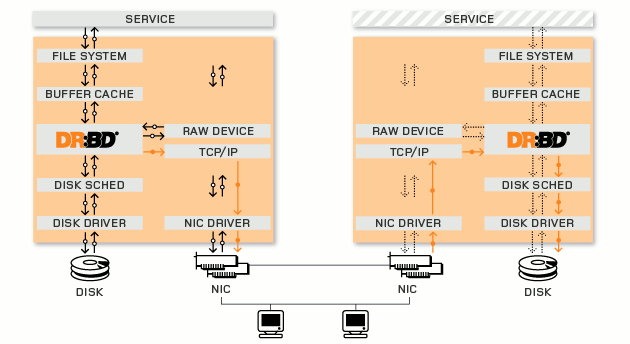
\includegraphics[keepaspectratio=true, width=\textwidth]{content/drbd.png}\\[1cm]
        
            \subsection{Installation}
                
                Pour la réplication bas niveau (système de fichiers), nous avons utilisé \underline{\href{http://www.drbd.org/}{DRBD}} : un logiciel permettant de faire de la réplication de données au sein d'une architecture en grappe. DRBD est assez complexe et fastidieux à mettre en place car il demande quelques notions assez poussées sur les volumes, leur synchronisations, etc.\\
                
                Ce logiciel ne fonctionnait autrefois qu'en mode maître/esclave mais depuis les dernières versions, on peut partir sur une configuration maître/maître afin que les données soient bien synchronisées de manière bidirectionnelle.\\
                
                \begin{bashcode}
                    # Installation de drbd
                    yum install -y drbd drbd-pacemaker drbd-udev
                \end{bashcode}
                
            \subsection{Configuration}
                
                La configuration de DRBD peu s'avérer très simple mais permet un certain degré de complexité en fonction des architectures. La syntaxe est claire et s'apparente à celle du serveur de nom.\\
                Voici la configuration que nous avons utilisé :\\
                
                \inputminted[
                    linenos=true,
                    bgcolor=lightgray,
                    tabsize=4,
                    fontfamily=courier,
                    fontsize=\small,
                    xleftmargin=5pt,
                    xrightmargin=5pt
                ]{bash}{./../confs/drbd/drbd.conf}
                
                DRBD implique qu'un lien réseau doit être établi en supplément des liens existants. Il est important de comprendre que le DRBD utilise un réseau à lui propre afin d'y transférer les données.\\
                
                Pour vérifier que DRBD fonctionne bien, il suffit de voir son état en faisant la commande suivante :\\
                
                \begin{bashcode}
                    cat /proc/drbd
                \end{bashcode}
                
        \section{Déploiement des services}
            
            Dans cette partie, il est important de comprendre que lors de la mise en place d'une architecture en grappe avec des noeuds répliqués, il faut toujours un noeud de référence, surtout dans une architecture active/passive comme celle que nous allons mettre en place.
            Suivant la machine sur laquelle vous allez lancer les scripts, il faudra ou non déployer les données.
        
            \subsection{Apache}
                
                \subsubsection{Installation}
                
                    Pour installer Apache, il vous faudra très simplement lancer son script d'installation dans le répertoire \verb+scripts/apache.sh+.
                    Ce script va essayer de stopper Apache, vérifier l'intégrité de son fichier de configuration et si il ne concorde pas avec le notre, il va le remplacer. Ensuite, selon si vous êtes le premier noeud de la grappe.
                
                \subsubsection{Configuration}
                    
                    La configuration d'Apache est très légèrement spécifique dû à notre application Web qui utilise \underline{\href{http://silex.sensiolabs.org}{Silex}} mais sinon rien de bien particulier ormis la configuration de l'URL \verb+/server-status+ qui doit être disponible pour Pacemaker.\\
                    
                    Il faudra donc bien décommenter le bout de code suivant à la fin du fichier :\\
                  
                    \begin{minted}[
                        linenos,
                        bgcolor=lightgray,
                        tabsize=4,
                        fontfamily=courier,
                        fontsize=\small,
                        xleftmargin=5pt,
                        xrightmargin=5pt,
                        gobble=24
                        ]{apache}
                        <Location /server-status>
                            SetHandler server-status
                            Order deny,allow
                            Deny from all
                            # Only from localhost where Pacemaker runs
                            Allow from 127.0.0.1
                        </Location>
                    \end{minted}
                    
                    Enfin, spécifier le \verb+DocumentRoot+ à \verb+/var/cluster/www/org/tp/g1b5/web+ et y ajouter les règles de réécritures suivantes afin de faire fonctionner notre application :\\
                    
                    \begin{minted}[
                        linenos,
                        bgcolor=lightgray,
                        tabsize=4,
                        fontfamily=courier,
                        fontsize=\small,
                        xleftmargin=5pt,
                        xrightmargin=5pt,
                        gobble=24
                        ]{apache}
                        <IfModule mod_rewrite.c>
                            Options -MultiViews
                            RewriteEngine On
                            # All requests which are not a file
                            RewriteCond %{REQUEST_FILENAME} !-f
                            # Except this request
                            RewriteCond %{REQUEST_URI} !=/server-status
                            RewriteRule ^ index.php [L]
                        </IfModule>
                    \end{minted}
                    
            \subsection{MySQL}
    
                \subsubsection{Installation}
                    
                    L'installation de MySQL se fait très facilement grâce au script d'installation \verb+scripts/mysql.sh+.\\
                    Le script arrête le serveur MySQL, charge le fichier de configuration \verb+confs/mysql/my.cnf+ à la place de l'ancien. 
Il démarre ensuite le service mysqld, puis cr\'ee les utilisateurs et peuple la base si nous sommes sur le premier noeud de la grappe.

                \subsubsection{Configuration}

                    Le fichier de configuration de MySQL est court, mais il est important dans notre cas de bien pr\'eciser le chemin du r\'epertoire ou seront 
stock\'ees les bases, \`a savoir dans notre cluster, dans le r\'epertoire \verb+/var/cluster/mysql+. De m\^eme, il est aussi important de pr\'eciser que 
l'adresse utilis\'ees par le serveur est celle de l'adresse du HAProxy : 10.192.10.50.\\

                    \inputminted[
                        linenos,
                        bgcolor=lightgray,
                        tabsize=4,
                        fontfamily=courier,
                        fontsize=\small,
                        xleftmargin=5pt,
                        xrightmargin=5pt
                    ]{ini}{./../confs/mysql/my.cnf}

                    Nous devons aussi d\'efinir le mot de passe de l'utilisateur ''root'', qui est le m\^eme sur les deux machines. Cela ce fait simplement 
gr\^ace \`a la commande :\\

                    \begin{minted}[
                        bgcolor=lightgray,
                        tabsize=4,
                        fontfamily=courier,
                        fontsize=\small,
                        xleftmargin=5pt,
                        xrightmargin=5pt,
                        gobble=24
                        ]{mysql}
                        mysqladmin password <mot_de_passe>
                    \end{minted}
                    
                    Il faut ensuite cr\'eer un utilisateur ``tpuser'', et lui allouer des droits de s\'election sur tout les machines du r\'eseau 10.192.10.0, 
afin de permettre l'acc\`es \`a la base ``projet\_hd'' depuis une machine distante.\\
                    
                    \inputminted[
                        linenos,
                        bgcolor=lightgray,
                        tabsize=4,
                        fontfamily=courier,
                        fontsize=\small,
                        xleftmargin=5pt,
                        xrightmargin=5pt
                    ]{sql}{./../confs/mysql/users.sql}

                    Il faut aussi cr\'eer puis initialiser la table ``product'', qui contient les donn\'ees sur notre stock. Elle contient les champs ``id'', ``name'', 
``price'' et ``quantity''.\\

            \subsection{DNS}

		    Pour commencer, il faut installer le paquet "<bind">. Comme pour les autres services, nous avons fait un script qui configure le serveur bind. 
Il copie tout simplement les fichiers de configuration que nous avons \'ecrit, puis lance le servic "<named">.\\

                    Nous avons choisi une configuration ma\^itre/esclave classique plutôt que d'utiliser DRBD et PaceMaker, car il n'y a pas de donn\'ees \`a r\'epliqu\'e 
comme avec k'annuaire LDAP ou MySQL, il y a seulement les fichiers de zones.\\

		    De m\^eme, pour les adresses des serveurs DNS, nous avons utilis\'e l'adresse des machines plut\^ot que celle du proxy. Le ma\^itre est donc la 
machine LLM, ayant l'adresse 10.192.10.24, et l'esclave la machine JB, 10.192.10.23.\\

		    Le fichier de configuration de bind est simple, et nous avons seulement rajout\'e la partie concernant les fichiers de zones. Dans les fichiers de 
zones, l'adresse des serveurs DNS est celle des machines correspondantes, mais l'adresse de "<g1b5.tp.org"> et celle des diff\'erents service est celle du proxy, 
10.192.10.50. \\

		    Nous n'avons pas pu donner d'adresses IPv6 aux diff\'erents services car Corosync et PaceMaker ne permettent pas de d\'efinir plusieurs adresses 
( ou du moins nous n'avons pas trouv\'e ) pour le proxy, les services ont donc seulement une adresse IPv4, seul les serveurs DNS ont une adresse IPv6.\\

		    FICHIER CONF BIND, FICHIERS DE ZONES

            \subsection{LDAP}

                    Il faut tout d'abord installer le paquets "<openldap">, puis lancer le script d'installation, qui remplace les fichiers de configuration pr\'esents 
sur la machine par les notres.\\

                    Pour configurer OpenLDAP, nous avons utilis\'e l'ancienne m\'ethode, avec le fichier "<slapd.conf">, plut\^ot que la nouvelle m\'ethode qui est 
tr\`es peu document\'ee. Il faut bien penser \`a supprimer le r\'epertoire \verb+/etc/openldap/slapd.d/+ car sinon OpenLDAP ne prend pas en compte le fichier "<slapd.conf">.\\

                    Le fichier "<ldap.conf"> contient seulement le suffixe de notre base :\\

                    FICHIER LDAP.CONF

                    Le fichier "<slapd.conf"> est quand \`a lui plus fourni :

                    FICHIER SLAPD.CONF

                    Ensuite le script peuple la base \`a l'aide d'un fichier .ldif. Nous stockons dans la base nos employ\'es, qui sont actuellement au nombre de deux, nous m\^emes.

                    FICHIER G1B5.LDIF

        \section{Mise en place de Pacemaker et Corosync}
            
            Dans une architecture HA, le système doit pouvoir constamment suivre son état et celui de son entourage afin de décider si il doit basculer (= ''failover'') ou non vers un noeud de secours. Pour cela, avec Fedora, nous avons choisi d'utiliser le service \underline{\href{http://clusterlabs.org}{Pacemaker}} couplé à \underline{\href{http://www.corosync.org}{Corosync}} car ils nous ont semblé très complets et très professionnels.
            
            \subsection{Présentation}
                
                Pour notre projet, nous avons choisi de mettre en place une architechure en grappes avec un système actif/passif. Ci-dessous un schéma de l'architechure :\\
                
                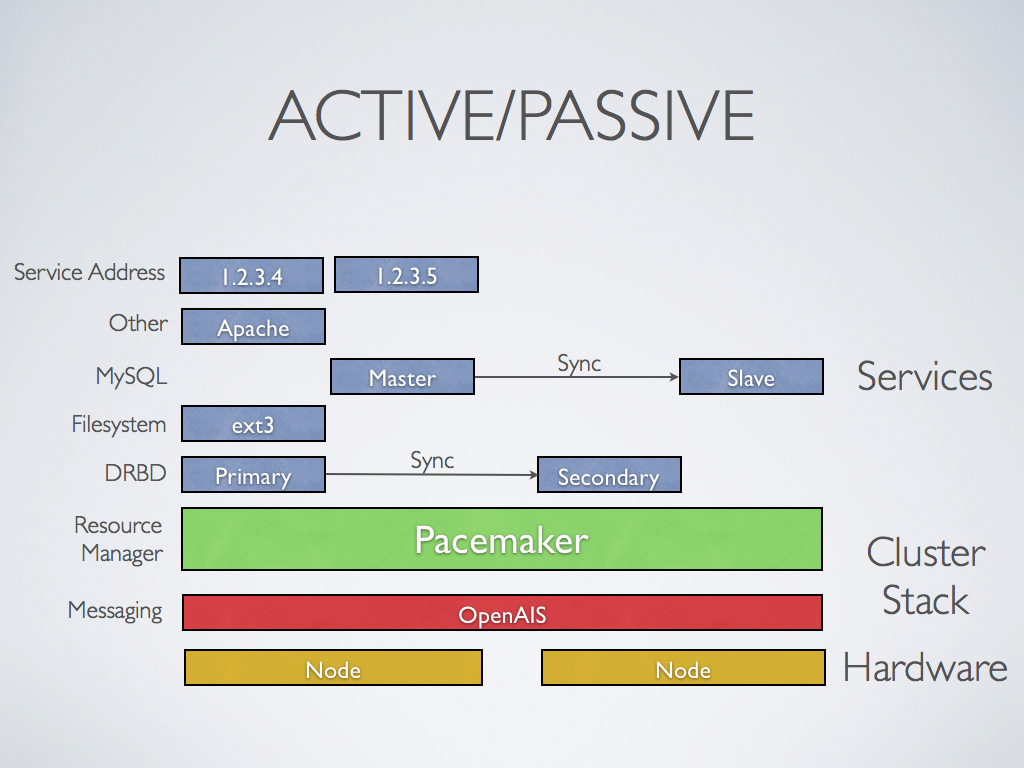
\includegraphics[keepaspectratio=true, width=\textwidth]{content/pacemaker-active-passive.png}\\[1cm]
                
                Les << node >> correspondent à nos machines (JB et LLM), la couche de messagerie OpenAIS correspondra au service Corosync qui est un projet dérivé d'OpenAIS. Pour les couches supérieures à Pacemaker, nous les avons vu précédemment.\\
                
                Corosync est un moteur de clustering mettant en oeuvre une messagerie de service sur réseau en utilisant une adresse et un port multicast.
            
            \subsection{Installation}
            
                \begin{bashcode}
                    # Installation de pacemaker et de corosync
                    yum install -y pacemaker corosync
                \end{bashcode}
            
            \subsection{Configuration}
                
                \subsubsection{Corosync}
                
                    Avant toute chose, voici les adresses IP nécessaires :\\

                    \begin{description}
                        \item[Adresse IP multicast] 239.0.0.1
                        \item[Port multicast] 6800
                        \item[Réseau de la grappe] 10.192.10.0
                        \item[Adresse IP de la grappe] 10.192.10.50
                    \end{description}

                    On va commencer par la configuration de Corosync qui est simpliste. Pour cela, on prends le fichier de configuration par défaut et on va simplement y changer les adresses IP comme ceci :\\

                    \begin{bashcode*}{gobble=24}
                        CONF="/etc/corosync/corosync.conf"
                        cp -f $CONF.example $CONF
                        sed -i.bak "s/.*mcastaddr:.*/mcastaddr:\ 239.0.0.1/g" $CONF
                        sed -i.bak "s/.*mcastport:.*/mcastport:\ 6800/g" $CONF
                        sed -i.bak "s/.*bindnetaddr:.*/bindnetaddr:\ 10.192.10.0/g" \$CONF
                    \end{bashcode*}

                    Ensuite, on va signaler à Corosync de charger le plugin Pacemaker afin qu'il puisse ''travailler'' avec :\\

                    \begin{bashcode*}{gobble=24}
                        cat << EOT > /etc/corosync/service.d/pcmk
                        service {
                                # Load the Pacemaker Cluster Resource Manager
                                name: pacemaker
                                ver:  1
                        }
                        EOT
                    \end{bashcode*}

                    Une fois configuré, nous pouvons lancer Corosync :\\

                    \begin{bashcode*}{linenos=false, gobble=24}
                        /etc/init.d/corosync start
                    \end{bashcode*}
                
                \subsubsection{Pacemaker}
                
                    Pacemaker offre une invite de commande propre à lui-même (comme les switch Cisco) que nous pouvons lancer en tapant \verb+crm+. Il est intéressant de savoir qu'en interne, la configuration de Pacemaker est formattée en XML car suite à quelques erreurs de notre part, nous avons pu constater des erreurs de validation d'entrée contre des Schémas XML.\\
                    
                    Afin de vous épargner la configuration à la main de Pacemaker, nous pouvons exporter et injecter directement une configuration donnée :\\
                    
                    \begin{bashcode*}{linenos=false, gobble=24}
                        crm configure load replace /path/to/conf/file
                    \end{bashcode*}
                    
                    Mais avant cela, vous devez démarrer Pacemaker et vider sa configuration actuelle (si existante) :\\
                    
                    \begin{bashcode*}{linenos=false, gobble=24}
                        /etc/init.d/pacemaker start
                        cibsadmin -E --force
                    \end{bashcode*}
                    
                    Voici donc notre fichier de configuration pour Pacemaker (la version initiale qui marchait correctement) :\\
                    
                    \inputminted[
                        linenos,
                        bgcolor=lightgray,
                        tabsize=4,
                        fontfamily=courier,
                        fontsize=\small,
                        xleftmargin=5pt,
                        xrightmargin=5pt
                    ]{text}{./../confs/pcmk/conf.work}
                    
                    Dans ce fichier, on peut y entrevoir des déclarations de ressources comme une IP ``flottante'' (\verb+10.192.10.50+) sur laquelle le monde extérieur va se connecter au services que contient la grappe, des ressources de battement de coeurs pour un système de fichier, les serveurs Apache, MySQL, LDAP et enfin la ressource de réplication bas niveau DRBD.\\
                    
                    Mais ce n'est que la déclaration des ressources, ensuite viennnent les dépendances de ``colocation'' qui obligent deux ressources données à toujours être de paire et enfin les ordres de démarrage des ressources en fonction des dépendances.
                    Par exemple, Apache ne peut pas démarrer avant que le système de fichier soit opérationnel.
            
                \subsection{Utilisation}
                
                    Pour \st{admirer} surveiller le bon fonctionnement de Pacemaker, il y a la commande \verb+crm_mon+.\\
                
                    En ce qui concerne la gestion des noeuds ou des ressources, il faut utiliser la commande \verb+crm+. Voici quelques exemples :\\
                
                    \begin{bashcode*}{gobble=24}
                        # Vérifier le status d'une ressource
                        crm resource status Apache
                        # Redémarrer une resource
                        crm resource restart MySQL
                        # Déplacer une ressource sur un autre noeud
                        crm ressource move FS mamba14
                        # Voir le status d'un noeud
                        crm node status mamba13
                        # Mettre un noeud en standby (simulation du failover)
                        crm node standby mamb14
                        # Et le rendre disponible à nouveau
                        crm node online mamba14
                    \end{bashcode*}

    \part{Tests}
        \section{Serveur de noms}
        \section{Serveur Apache}
        \section{Serveur MySQL}
        \section{Serveur LDAP}
    \part{Conclusion}
        \section{Difficultés rencontrés}
            
            Durant ce projet, la contrainte majeur était de réaliser une telle architechure en 3 jours seulement sans avoir aucune expérience dans le domaine. Nous avons souhaité nous orienter vers des choix fonctionnels et matures plutôt qu'universitaires et peu professionnels.\\
            
            Le premier facteur de difficulté aura été l'abscence d'indications concernant le choix des technologies car nous avons réellement été soumis à un environnement pragmatique où nous jouons le rôle des responsables SI vers qui on vient se conseiller suite une problématique bien présente.
            Le choix et la décision des technologies est une chose mais ce qui est le plus chronophage est de regarder les produits et les solutions existantes sur le marché.\\
            
            Une fois les choix réalisés, il a fallu se documenter pour savoir implémenter au mieux possible l'infrastructure logicielle. Nous ne vous cacherons pas que nous avons lu 90\% de documentation en anglais durant ces 3 jours. De l'anglais pas toujours facile à comprendre de part ses termes techniques mais surtout de part la notion nouvelle que nous découvrions sur le tas.\\
            
            La difficulté suivante fut liée aux machines elles-même : impossible de prévoir que tout va fonctionner du premier coup, le fait que les machines aient besoin d'un serveur mandataire pour accèder au Web rajoute quelques contraintes sur les configurations mais surtout le manque de maîtrise complet sur les distributions Fedora nous aura fait perdre un peu de temps non négligeable.\\
            
            Malgré tout cela, nous sommes parvenus automatiser de manière relativement complète l'installation, la configuration et le déploiement de notre projet à l'aide de Subversion et de scripts Bash.
        
        \section{Retours sur échec}
        
            Après 3 jours de recherche, de développement et de tests acharnés sur les différentes briques de notre architechure, nous avons échoué lors de la présentation de notre projet. En voici les raisons majeures :\\
            
            \begin{enumerate}
                \item Manque d'expérience avec les technologies utilisées
                \item Manque d'organisation et de rigueur dans les procédures
                \item Manque de temps (implique du stress)
                \item Analyses sur tests défaillants pas assez complètes
            \end{enumerate}
            
            D'une certaine manière, tous ces facteurs sont liés car ils s'entre-croisent et s'encouragent et nous le savions mais pas c'est pas toujours évident d'avoir le temps de prendre le recul nécessaire afin de mieux repartir.\\
            
            Après des heures intensives de travail, nous avions réussi à faire tourner notre architechure active/passive en simulant des failovers et des failback avec succès mais sans tester tous les cas possibles et surtout les cas d'évaluation. Suite à ce succès précipité, nous avons voulu optimiser la configuration de Pacemaker afin de la simplifier mais nous nous sommes rendu compte après analyse que cette nouvelle configuration ne répondait plus au contraintes d'ordre de basculement des services lors du failover.
            
            Dans le stress et la précipitation, nous avons voulu essayer une architechure active/active car nous pensions que le type d'architechure active/passive ne répondait pas à la demande de l'évaluation (analyse d'échec pas assez poussée) mais près quelques heures d'installation et de configuration, cette nouvelle monture n'a pas été un succès à cause d'un soucis de synchronisation de volume avec DRBD bien que la nouvelle configuration active/active de Pacemaker était déjà prète.
        
        \section{Retours personnels}
\end{document}